\chapter{Administrator's guide} 
\label{chap:admin} 

The core generic package contains tightly-optimized, multithreaded posterior prediction code that works for a wide variety of PyMC probability models. This code is used primarily by \texttt{mbg-validate} and \texttt{mbg-map}. The package depends completely on PyMC for the Markov chain Monte Carlo algorithm needed by \texttt{mbg-infer}. These shell commands are described in detail in chapter \ref{chap:user}.

The core package is adapted to each scientific situation by means of a `specializing module'. The specializing modules are plain Python packages, complete with \texttt{setup.py} scripts, that expose certain attributes. These attributes are documented in detail in chapter \ref{chap:stat}.

\begin{figure}[hhh]
    \begin{center}
        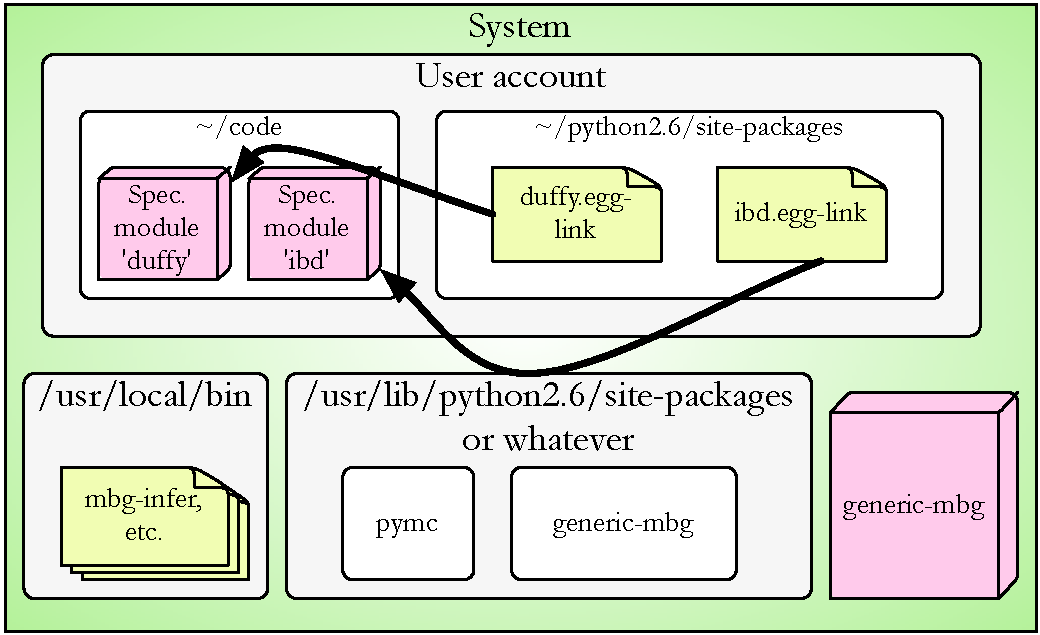
\epsfig{file=installation.pdf, width=10cm} 
    \end{center}
    \caption{The overall installation scheme. The \texttt{generic\_mbg} and \texttt{PyMC} packages are installed to the system-wide \texttt{site-packages} directory, and the executables \texttt{mbg-infer}, \texttt{mbg-map} etc. are installed to \texttt{/usr/local/bin}. The specializing modules are installed locally to user accounts using the \texttt{develop} command (see section \ref{sec:spec-local}). This command places a link to the source code in the user's \texttt{site-packages} directory, so the user can alter the code in-place the changes will take effect immediately. Git repositories are shown as pink boxes. The \texttt{generic-mbg} package and the specializing modules must be git repositories, because the commit hashes of both are stored in the MCMC trace to avoid versioning confusion. Yellow pages are flat files.   }
    \label{fig:installation}
\end{figure}

\bigskip
This chapter explains how to install and maintain the core package and the specializing modules at an IT level, and how to administer user accounts. The overall installation scheme is illustrated in figure \ref{fig:installation}.

\bigskip
Before reading this chapter, you should become familiar with \href{http://docs.python.org/install/index.html}{Python's library management system}.

\section{Dependencies}

The following top-level dependencies should be available from most package managers. Be sure to install the package corresponding to the correct version of Python:
\begin{itemize}
    \item \href{http://pypi.python.org/pypi/setuptools}{Setuptools} 
    \item \href{http://rpy.sourceforge.net}{RPy} is required by \texttt{mbg-decluster} only. 
    \item \href{http://www.pytables.org}{PyTables}
    \item \href{http://matplotlib.sourceforge.net}{Matplotlib}  
    \item \href{http://www.scipy.org}{SciPy} 
\end{itemize}

After those packages are installed, \href{http://code.google.com/p/pymc}{PyMC} needs to be installed. As of this writing it should be checked out from either the Google Code subversion repository or \href{http://github.com/pymc-devs/pymc}{github} and built from source. See the PyMC user guide for details on PyMC's dependencies and installation instructions.

Finally, the following MAP packages should be checked out and installed from source:
\begin{itemize}
    \item \href{http://github.com/malaria-atlas-project/map_utils}{The utilities package} 
    \item \href{http://github.com/malaria-atlas-project/st-cov-fun}{The space-time covariance function package} This shouldn't be a core dependency, I'll remove it when I get the chance.
\end{itemize}

\section{Installing the generic package}
The generic package lives at \href{http://github.com/malaria-atlas-project/generic-mbg}{MAP's github repository}. The procedure for installing the package is as follows:

\begin{verbatim}
    git clone git://github.com/malaria-atlas-project/generic-mbg.git
    cd generic-mbg
    sudo python setup.py install
\end{verbatim}

The package has to be installed from a local clone of the repository (rather than a simple download of the code), because it will include the git commit hash in the executables it installs. The executables, in turn, will store the commit hash in each trace file, so that there is a record of which version of the generic package produced all products.

\subsection{Local installation to a user account}
\label{sub:core-local} 
By default, the executables are installed to \texttt{/usr/local/bin}. The setup script can be instructed to make a local installation in a user's account, if the user requires a special version of the generic package. The local installation scheme is illustrated in figure \ref{fig:local-installation} 

In this case, the installation should be done as the user (rather than as \texttt{su}):
\begin{verbatim}
    python setup.py install --install-dir=~/ros/python2.6/site-packages
       --executable-dir=~/ros/bin 
\end{verbatim}
The \texttt{executable-dir} argument is specific to this package. The \texttt{install-dir} argument is used by setuptools. Be sure to add the executable directory to the user's path!

\begin{figure}[hhh]
    \begin{center}
        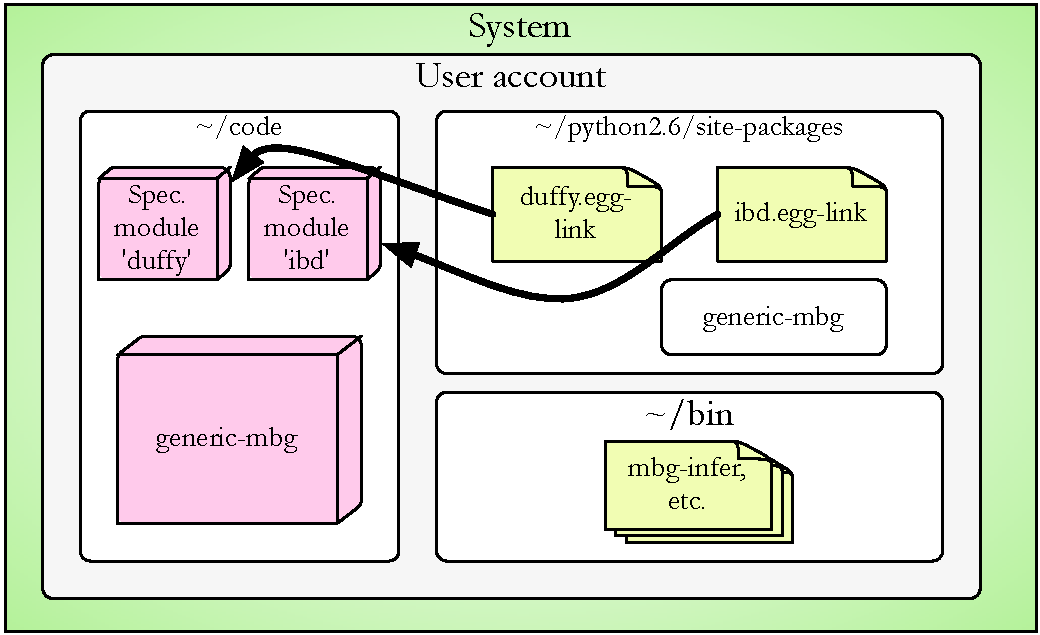
\epsfig{file=installation-local.pdf, width=10cm} 
    \end{center}
    \caption{Local installation to a user account. The \texttt{generic-mbg} package is installed to the local \texttt{site-packages} directory alongside the specializing modules, and its executables are written to the local \texttt{bin} directory. PyMC is still installed system-wide. As in figure \ref{fig:installation}, pink boxes are git repositories and yellow pages are files.}
    \label{fig:local-installation}
\end{figure}

\section{Installing the specializing modules}
\label{sec:spec-local} 
Like the core package, the specializing modules need to be installed from local git repositories. The commit hash of the specializing module is stored in each trace along with the commit hash of the generic package, in order to avoid future versioning problems.

\medskip
Specializing modules must be installed using the \texttt{develop} command rather than the \texttt{install} command. The \texttt{install} command actually copies the package source, and all compiled extensions, to the \texttt{site-packages} directory. The \texttt{develop} command, on the other hand, only puts a link to the source directory in the \texttt{site-packages} directory. The result is that changes to the source directory are automatically `installed'.

The specializing modules need to be installed using \texttt{develop} to make it easier for users to make small changes on their own, and because of the way the core package looks for the specializing modules' commit hashes. Remind users to commit to their local clone of the repository before running any MCMC's, to be sure the versioning information gets recorded correctly.

The procedure for installing a specializing module, say \texttt{duffy}, is:
\begin{verbatim}
    git clone git://github.com/malaria-atlas-project/duffy.git
    cd duffy
    python setup.py develop --install-dir=~/ros/python2.6/site-packages
\end{verbatim}
The \texttt{install-dir} argument tells setuptools where to put the link. Be sure to add the installation directory to the user's \texttt{PYTHONPATH}, preferably ahead of the system-wide \texttt{site-packages} directory. The installation should be run as the user, not as \texttt{su}.

\section{Environment variables}
The following environment variables affect the functioning of the generic package:
\begin{description}
    \item[PATH] Should include the executable directory in section \ref{sub:core-local}.
    \item[PYTHONPATH] Should include the \texttt{site-packages} directories in sections \ref{sub:core-local} and \ref{sec:spec-local}. The one in \ref{sec:spec-local} should come first.
    \item[OMP\_NUM\_THREADS] Sets the maximum number of CPU cores available to the package's operations. 
\end{description}

\section{Explaining to users how to work in UNIX-like environments}

In addition to the standard UNIX commands (\texttt{mv}, \texttt{cp}, etc.) be sure to explain \texttt{ssh}, \texttt{scp} and most especially \texttt{screen}. Screen is completely indispensable for people who are launching long compute jobs from Windows machines that reboot themselves frequently, and for people with unreliable internet connections.

I sent the following email around to the users about keeping out of each other's way, you may want to send something similar:

\bigskip
{\sffamily

It's a very good thing that multiple factions of MAP are now empowered to run their own geostatistical analyses without going through Pete and I (and, god forbid, IRIDIS). However, we all need to be considerate in order to avoid adversely affecting each other's jobs.


Here are the linux commands that will help you do that:

\begin{itemize}
    \item \texttt{top} shows all the processes running on a given machine. Here's an example top output from my mac:

    \begin{verbatim}
    Processes:  129 total, 3 running, 6 stuck, 120 sleeping... 801 threads                                              17:45:47
    Load Avg:  5.28,  3.04,  2.55    CPU usage: 76.29% user,  7.04% sys, 16.67% idle
    SharedLibs: num =    8, resident =   57M code,  692K data, 4472K linkedit.
    MemRegions: num = 50361, resident = 2310M +   31M private,  412M shared.
    PhysMem:  740M wired, 3926M active,  707M inactive, 5377M used, 2815M free.
    VM: 21G + 374M   635726(0) pageins, 657247(0) pageouts

      PID COMMAND      %CPU   TIME   #TH #PRTS #MREGS RPRVT  RSHRD  RSIZE  VSIZE
    77589 DashboardC   0.0%  0:06.73   5   152    596   25M    15M    40M   437M 
    75546 iTunes       0.0% 62:23.59  35   580    818   24M    30M    63M   501M 
    73904 ssh          0.0%  0:00.09   1    15     27   84K   444K   748K    19M 
    72628 ForkLift     1.2%  2:19:07  22   199    542   44M    23M    58M   481M 
    70321 Preview      0.0%  2:06.58  28   214    462   15M    14M    17M   433M 
    58862 TextMate     0.0% 13:45.74 101   392   1336  496M    67M   599M  1620M 
    56142 VoodooPad    0.0% 13:23.72  20   162    425 1516K    12M  7568K   427M 
    46574 smbtree      0.1%  0:00.05   1    13     37  484K   184K  1436K    20M 
    46555 Python     586.4% 10:01.92   9    56-   707  728M- 2988K   735M-  917M-
    46333 Python       0.0%  0:00.53   1    14    199 8608K  2656K    11M    27M 
    43464 bash         0.0%  0:00.00   1    14     19  244K   680K   884K    18M 
    43300 mdworker     0.0%  2:15.63   4    76    197 4820K  6192K    14M    83M     
    \end{verbatim}

    Notice process number 46555, which is a mapping job. It's using 586.4\% of the CPU right now. That means it's using about six of this machine's eight cores. 

    If you start another mapping job on my machine, the two will compete for resources, meaning they'll both slow down. This slowdown is usually nonlinear. Like humans, processor cores are more efficient when they can concentrate on a single task rather than switching contexts all the time.

    On the other hand, if you start a small job, such as an MCMC with n less than 100, my mapping job probably won't notice the difference, because my computer has spare capacity.

    Top can also show only the processes owned by particular users, for example:

    \begin{verbatim}
    top -U anand
    top -U noor
    top -U ibd    
    \end{verbatim}


    \item If you want start a long, heavy-duty job, but don't need the results in a hurry, you can tell the operating system to de-prioritize it with the \texttt{nice} command. Then, if someone else starts a job, the OS will take resources away from your job to give to it.

    Normally, you would start a mapping job with:

    \begin{verbatim}
    mbg-map module etc. etc.    
    \end{verbatim}

    To start it at low priority, do:

    \begin{verbatim}
    nice mbg-map module etc. etc.    
    \end{verbatim}


    If you start a job but then realize later that you want it to run at low priority, you can use renice. Renice needs to know the process id (PID) of the job, which you can get from top. For example, to deprioritize my mapping job, I would do

    \begin{verbatim}
    renice -p 46555    
    \end{verbatim}



    \item If you're using a lot of disk space, please download some of your stuff and delete it on the server. The linux machine has very limited disk space. The macs have 1TB each, but we'll fill them up pretty quickly anyway.

    To figure out how much disk space you're using, use the command \texttt{du}. Du will tell you how much disk space is being used by all subdirectories within the current directory. The last number it tells you is the total disk space used in the current directory. For example:

    \begin{verbatim}
    du 

    688     ./build/temp.macosx-10.5-i386-2.5/build
    16      ./build/temp.macosx-10.5-i386-2.5/generic_mbg

    ...

    712     ./test/ke_test-plots
    1477000 ./test/ke_test-validation
    1492064 ./test
    1496352 .    
    \end{verbatim}

    It looks like the current directory is using 1,496,352 kb, or about 1.5 gb. Most of that seems to be in the \texttt{test} subdirectory. To get more detail and see how much space each individual file uses, use du -a
\end{itemize}
}

\section{Compiled extensions}

The core package and many of the specializing modules contain Fortran code. A C wrapper binding the Fortran code to the Python-C API is generated by the NumPy subpackage f2py, and the lot is compiled by setup.py

It's relatively common to see problems in the compiled extensions, either compile-time errors or runtime linking errors, that are caused by inappropriate compiler flags. Pay special attention to the \texttt{CFLAGS}, \texttt{FFLAGS} and \texttt{LDFLAGS} environment variables.

\section{\texttt{mbg-init-user-account}}

The shell command \texttt{mbg-init-user-account} automates the setup of user accounts. The command
\begin{verbatim}
    mbg-init-user-account duffy git://github.com/malaria-atlas-project/duffy.git
        mbg-world git://github.com/malaria-atlas-project/mbg-world.git
\end{verbatim}
run as a new user would have the following effects:
\begin{itemize}
    \item Directories \texttt{\~/code}, \texttt{\~/bin}, \texttt{\~/python2.6/site-packages} created
    \item Specialization modules \texttt{duffy} and \texttt{mbg-world} cloned from the prodvided URL's into \texttt{\~/code} and installed to \texttt{\~/python2.6/site-packages}
    \item Standard versions of \texttt{\~/.matplotlib/matplotlibrc} and \texttt{\~/.ipython/ipythonrc}
    \item Extra environment variables added to the RC file, \texttt{.bashrc} for Linux machines or \texttt{.Profile} for macs.
\end{itemize}
However, there's no way we can make this shell command work globally; chances are very good that you'll have to manually make some changes to RC files.